\documentclass[11pt]{article}

\usepackage[a4paper,margin=1in]{geometry}
\usepackage[utf8]{inputenc}
\usepackage[T1]{fontenc}
\usepackage{times}
\usepackage{microtype}
\usepackage{graphicx}
\usepackage{amsmath,amssymb}
\usepackage{booktabs}
\usepackage{natbib}
\usepackage{hyperref}
\usepackage{authblk}
\usepackage{lineno}

\hypersetup{colorlinks=true, linkcolor=blue!50!black, citecolor=blue!40!black,
            urlcolor=blue!40!black}

\title{\textbf{miniML: A Deep Learning Framework for Automated and Generalized Synaptic Event Analysis}}
\author[1]{Anonymous Author(s)}
\affil[1]{For submission to \textit{eLife}}
\date{}

\begin{document}

\maketitle
\linenumbers

\begin{abstract}
\noindent
Quantitative information about synaptic transmission is central to our
understanding of neural function, and spontaneously occurring synaptic events
are one of the most direct experimental windows onto that function. Their
stochastic occurrence and low signal-to-noise ratio, however, make
reliable, operator-independent detection difficult. We present miniML, a
supervised deep learning framework for the accurate classification and
automated detection of spontaneous synaptic events. A compact convolutional-
recurrent classifier, trained on roughly 30{,}000 labeled segments of mouse
cerebellar mossy fiber to granule cell miniature excitatory postsynaptic
currents, reaches 98.4\% validation accuracy. Applied with a sliding-window
inference procedure it detects events in arbitrarily long recordings with
close-to-zero false positive rates and with detection performance that is
virtually insensitive to threshold choice. On synthetic ground-truth data
miniML delivers the highest F1 score across the full range of signal-to-noise
ratios seen in miniature-event recordings, outperforming template matching,
deconvolution, finite-threshold detection, Bayesian inference, SimplyFire, and
commercial MiniAnalysis software. Using a transfer learning strategy that
freezes the convolutional feature extractor, miniML generalizes from mouse
cerebellum to the Calyx of Held, cerebellar Golgi cells, human iPSC-derived
cortical neurons, adult zebrafish telencephalon, \textit{Drosophila}
neuromuscular junctions, iGluSnFR3 glutamate imaging, and ASAP5 voltage
imaging, in each case matching or exceeding the best alternative method. In
the low-SNR optical regime miniML is the only method that recovers a
substantial fraction of the ground-truth events (F1 = 0.53 $\pm$ 0.04 vs.\
0.39 $\pm$ 0.05 for template matching and 0.17 $\pm$ 0.01 for deconvolution).
A detector with these four properties, accurate, automated, robust to
threshold choice, and readily retargetable via transfer learning, is the
enabling piece of infrastructure that high-throughput, reproducible
analysis of synaptic function and dysfunction has been waiting for across
species and recording modalities.
\end{abstract}

% ----------------------------------------------------------------------------
% Introduction and Related Work
% ----------------------------------------------------------------------------
\section{Introduction}

Synaptic communication is the substrate for essentially every computation the
brain performs, from sensory integration through working memory and motor
control. Most of that communication is carried by discrete synaptic events:
brief, stereotyped postsynaptic responses that follow the fusion of single
neurotransmitter-filled vesicles \citep{kaeser2014release}. A sizeable
fraction of these events occur spontaneously, independent of presynaptic
action potentials, and these ``miniature'' events are far more than
background noise. Their amplitude, frequency, and kinetics are a direct
readout of receptor composition, presynaptic release probability, and the
functional state of a synapse \citep{kavalali2015mechanisms, huganir2013ampars,
reese2015spontaneous}. Changes in miniature-event statistics accompany
homeostatic scaling, Hebbian plasticity, and many disease states across model
systems, and their quantitative analysis underpins much of modern cellular
neurophysiology.

Despite their centrality, detecting and quantifying individual synaptic events
in raw recordings remains stubbornly difficult. The events themselves are
small relative to background noise, their timing is stochastic, and their
waveform depends on the recording configuration, the receptor complement, the
developmental stage of the preparation, and even the sampling hardware. The
dominant algorithmic responses to these difficulties fall into three families.
Finite-difference methods detect threshold crossings in the raw trace or in
its derivative; template-matching methods convolve the trace with a
stereotyped event waveform and look for peaks in the resulting score
\citep{clements1997detection}; and deconvolution methods invert a template to
concentrate each event into a narrow impulse that is easier to threshold
\citep{pernia2012deconvolution}. Bayesian inference procedures treat event
times and amplitudes as latent variables and estimate them jointly under a
generative model \citep{merel2016bayesian}. Each of these approaches works
well in some regime and fails in another. Finite-threshold methods are simple
but exquisitely sensitive to noise. Template-based methods require the user to
supply (or tune) a waveform that closely matches the real events, and their
output depends strongly on a user-chosen threshold. Bayesian methods are
powerful but computationally expensive and require careful prior
specification. In practice, many laboratories still rely on manual inspection
or proprietary software \citep{mori2024simplyfire} to curate detected events,
which introduces investigator-dependent variability that is incompatible with
large-scale, reproducible analysis.

Deep learning has reshaped the way noisy, high-dimensional biological signals
are processed \citep{lecun2015deep}. Convolutional neural networks excel at
one-dimensional signal classification, and sequence models such as long
short-term memory networks can capture the temporal structure of the
surrounding context \citep{fawaz2019deeptsc}. In neuroscience specifically,
CNN-based approaches now dominate spike inference from calcium imaging
\citep{rupprecht2021cascade}, and transfer learning from large pretrained
models is rapidly becoming the standard recipe for adapting a network trained
on abundant data to a new domain with only limited labeled examples
\citep{theodoris2023transfer, yosinski2014transferable}. These same
ingredients, end-to-end learning, transfer, and automatic feature extraction,
are a natural fit for spontaneous synaptic event detection, yet the community
lacks an open, systematically benchmarked tool that delivers them in a form a
wet-lab electrophysiologist can actually use.

Here we introduce miniML, a supervised deep learning framework for the
automated, reproducible, and highly generalizable detection of synaptic
events. miniML couples a compact CNN-LSTM classifier to a sliding-window
inference procedure. It is trained on roughly 30{,}000 labeled segments from
mouse cerebellar MF-GC mEPSC recordings, and then either applied directly to
similar data or rapidly adapted to new preparations via transfer learning
with as few as 400 labeled events. Against a panel of six established methods
on synthetic ground-truth data, miniML delivers the highest F1 across the
full range of signal-to-noise ratios encountered in real miniature-event
recordings, exhibits no false positives in the tested regime, and is
virtually insensitive to threshold choice. It generalizes from mouse
cerebellar slices to the Calyx of Held, human iPSC-derived cortical neurons,
adult zebrafish telencephalon, \textit{Drosophila} neuromuscular junctions,
and optical imaging data acquired with both the glutamate sensor iGluSnFR3
\citep{aggarwal2023iglusnfr3} and the voltage indicator ASAP5
\citep{hao2024asap5}. In each of these settings miniML either matches or
exceeds the detection performance of the best alternative method, and in the
low-SNR voltage-imaging regime it is the only method that recovers a
substantial fraction of the ground-truth mEPSPs.

\section{Related Work}

\paragraph{Classical detection of spontaneous synaptic events.}
The two most widely used algorithms, sliding-template matching
\citep{clements1997detection} and deconvolution
\citep{pernia2012deconvolution}, have defined the field for more than two
decades. Both require a fixed template that represents the expected event
waveform. When the template is well matched to the data, they are sensitive
and fast; when event kinetics drift because of a different preparation,
receptor composition, or recording mode, their performance degrades and,
critically, their output is strongly modulated by the chosen detection
threshold. Finite-difference methods \citep{kudoh2002template} are simpler
still but push the burden of noise rejection entirely onto the threshold.
More recent tools such as SimplyFire \citep{mori2024simplyfire} provide
usable GUIs and sensible defaults on top of these classical ideas, but they
inherit the same structural limitations.

\paragraph{Probabilistic event inference.}
Bayesian approaches frame event detection as inference in a generative model
of the recording \citep{merel2016bayesian}. This confers robustness to noise
and a principled way to combine electrophysiological traces with auxiliary
observations such as simultaneous optical reporters. The cost is
computational: MCMC procedures are orders of magnitude slower than
convolutional detectors, which makes them unattractive for analyzing the
minutes-long recordings typical of miniature-event experiments.

\paragraph{Deep learning for one-dimensional neurophysiological signals.}
Deep learning broke into neuroscience through imaging and spike inference
\citep{lecun2015deep, rupprecht2021cascade}, and recent reviews of
one-dimensional time-series classification show that CNN-LSTM architectures
routinely outperform hand-engineered baselines on a wide variety of biological
signals \citep{fawaz2019deeptsc}. Transfer learning, in which a model trained
on a data-rich source task is partially reused on a target task, has become a
standard recipe \citep{yosinski2014transferable, theodoris2023transfer}.
miniML is, to our knowledge, the first open framework to bring this
combination, an end-to-end CNN-LSTM classifier plus transfer learning, to
spontaneous synaptic event detection, and to systematically benchmark it
against both classical and probabilistic baselines on shared synthetic
ground-truth data.

\paragraph{Optical detection of synaptic events.}
The recent generation of genetically encoded indicators, in particular
iGluSnFR3 for glutamate \citep{aggarwal2023iglusnfr3} and ASAP5 for membrane
voltage \citep{hao2024asap5}, has made it feasible to record unitary synaptic
events with cellular and subcellular resolution. These recordings are,
however, substantially noisier than patch-clamp electrophysiology and have a
much lower sampling rate, which exposes the weaknesses of template-matching
and deconvolution methods that were designed for high-SNR current traces. A
detector that tolerates slower kinetics, lower SNR, and variable noise
profiles is therefore an increasingly pressing need, and precisely the gap
that miniML targets.

% ----------------------------------------------------------------------------
% Results
% ----------------------------------------------------------------------------
\section{Results}

We present miniML's performance in seven steps: first the classifier itself,
then the sliding-window detector built on top of it, a head-to-head
benchmark against six established methods, transfer across preparations and
species, detection at the \textit{Drosophila} neuromuscular junction, and
finally optical detection with iGluSnFR3 and ASAP5. Throughout, numerical
values are given as mean $\pm$ SD unless noted otherwise.

\subsection{miniML accurately classifies short segments of electrophysiological data}

We posed synaptic event detection first as a classification problem: given a
short segment of a voltage-clamp or current-clamp recording, does it contain
a synaptic event? The classifier must be selective enough to reject noise
excursions with event-like shape and robust enough to tolerate the variable
baselines, occasional transients and pharmacological perturbations that are
routine in real recordings. We therefore designed a small convolutional-
recurrent network (miniML, Figure~\ref{fig:arch}) in which three 1D
convolutional blocks, each a convolution followed by a leaky-ReLU activation,
batch normalization \citep{ioffe2015batchnorm} and average pooling, extract
local time-domain features. A fourth convolutional block without pooling
preserves temporal resolution, the output is passed through a bidirectional
long short-term memory layer that integrates information across the window,
and a fully connected layer with dropout \citep{srivastava2014dropout}
produces a single sigmoid output in $[0,1]$. The architecture contains
190{,}913 trainable parameters.

Training data came from voltage-clamp recordings of miniature excitatory
postsynaptic currents (mEPSCs) at the mouse cerebellar mossy fiber to granule
cell (MF-GC) synapse. Event-containing and event-free segments of 600 samples
(12~ms at 50~kHz) were extracted, manually curated, and balanced
approximately 1:1 to yield a final training set of 30{,}140 samples (21{,}140
from recordings and 9{,}000 simulated), which was split 0.75/0.25 into
training and validation partitions. The network was optimized with Adam
\citep{kingma2014adam} at a learning rate of 2$\times 10^{-5}$ and batch
size 128, with early stopping (patience 8) on the validation loss. The
best-performing model reached a binary accuracy of 98.4\% (SD 0.1) over
fivefold cross-validation, with the gap between training and validation
accuracy held below 0.3\% by the early-stopping rule
(Figure~\ref{fig:arch}). The area under the receiver operating characteristic
was near unity, and saliency-map analysis \citep{simonyan2013saliency}
confirmed that the classifier concentrated its discriminative evidence on the
event peak, exactly where an electrophysiologist would look. Uniform manifold
approximation and projection of the penultimate layer activations shows a
nearly linear separation of the two classes.

To understand how much training data the architecture actually needs, we
systematically subsampled the MF-GC dataset and retrained with fivefold
cross-validation. Accuracy increased smoothly with dataset size up to a few
thousand samples; beyond 5{,}000 samples the gain was marginal, less than
0.2\% in binary accuracy. This result is practically important: it tells the
experimentalist that a training corpus of a few thousand hand-labeled
segments is sufficient to train a classifier of this architecture from
scratch, which brings the method within reach of most electrophysiology
laboratories.

\subsection{A sliding-window procedure turns the classifier into a detector}

Synaptic events occur at times unknown to the experimenter, and the duration
of a typical recording (here 120~s at 50~kHz, i.e.\ six million samples)
forbids classifying every possible window. We therefore applied the trained
classifier with a sliding window of 600 samples and a stride that trades
temporal precision against inference cost. Stride values up to 5\% of the
window size left detection performance effectively unchanged, and a stride
of 20 samples let a 120~s recording be analyzed in roughly 15~s on a laptop
(Apple M1 Pro, 16~GB RAM); GPU acceleration brought the wall-time below
20~s for the same 6{,}000{,}000-sample trace. The output of the network is a
prediction trace, resampled to the acquisition sampling rate, whose value at
each time point is the classifier's confidence that the surrounding window
contains an event. Peaks above a minimum height of 0.5 and a minimum width
of ten strides mark candidate events; the exact numerical peak-height
threshold proves to be largely irrelevant, as we show below. Each candidate
is aligned by its point of steepest rise, overlapping events are split using
a relative-prominence criterion of 0.25, and individual event amplitudes,
rise times (10-90\%), half-decay times, and charges are quantified directly
from the aligned raw data.

\subsection{Systematic benchmarking demonstrates superior performance across SNRs}

We next compared miniML against six independent event-detection methods: the
Clements-Bekkers sliding template \citep{clements1997detection}, deconvolution
\citep{pernia2012deconvolution}, a finite-threshold detector
\citep{kudoh2002template}, a Bayesian MCMC procedure
\citep{merel2016bayesian}, the open-source peak-finder SimplyFire
\citep{mori2024simplyfire}, and the commercial MiniAnalysis software. To
avoid the biases inherent in hand-labeled ground truth we generated
standardized benchmark data by superimposing simulated events onto
pharmacologically silenced, event-free voltage-clamp recordings from mouse
cerebellar granule cells. Simulated events used a two-exponential waveform,
amplitudes drawn from a log-normal distribution with variance 0.4, decay time
constants drawn from a normal distribution with mean 1.0~ms and variance
0.25~ms, and an average event rate of 0.7~Hz with a 3~ms minimum spacing. By
scaling the mean amplitude we covered the signal-to-noise range seen in a
cohort of 170 real MF-GC recordings (roughly 2-15~dB).

Across this range, recall depended strongly on SNR for every method, but
miniML and deconvolution led the pack; precision was uniformly highest for
miniML, which contributed no false positives at any SNR, whereas every other
method produced at least some. Overall F1 was highest for miniML across the
entire tested SNR range. When we perturbed the simulated event kinetics to
decouple them from the benchmark template, template matching, deconvolution,
and the Bayesian detector all lost ground, while miniML remained robust:
recall exceeded 80\% for events with kinetics up to roughly four times
slower than the training distribution.

A more subtle consequence of moving from a hand-tuned template to a learned
classifier concerns the detection trace itself. Classical methods produce a
trace with the same arbitrary units as the data, in which peak height
correlates strongly with event amplitude. The detection threshold therefore
doubles as an amplitude cutoff, and a small change in threshold moves the
population of detected events in ways the user cannot easily predict.
miniML, in contrast, outputs a bounded confidence in $[0,1]$ whose peaks are
effectively decorrelated from event amplitude. Sweeping the miniML threshold
from 5\% to 195\% of its default value left the number of detected events
and the F1 score nearly unchanged over almost the full range; false
positives appeared only at the 5\% extreme (a cutoff of 0.025 in the
detection trace). For every alternative method except the Bayesian detector,
the analogous threshold sweep produced dramatic changes in both metrics.
The combination, high precision, high recall, and very weak threshold
dependence, is the core empirical advantage of miniML over existing
approaches.

\subsection{miniML generalizes to out-of-sample preparations}

A detector trained on one synapse is only useful if it transfers. We
therefore applied the pretrained MF-GC model, unchanged, to voltage-clamp
recordings from four qualitatively different preparations. At the mouse
Calyx of Held, a large auditory-brainstem synapse with very fast event
kinetics, miniML detected spontaneous mEPSCs robustly despite never having
seen such data during training. At cerebellar Golgi cells, whose synaptic
events are substantially slower (half-decay 1.83~ms, SD 0.44~ms, n = 10
neurons, against 0.9~ms in the MF-GC training data), a larger analysis
window of 900 samples sufficed to maintain detection quality. In cultured
human iPSC-derived cortical glutamatergic neurons, miniML recovered
spontaneous EPSCs in the roughly 51\% of cells in which such events were
present, yielding a mean frequency of 0.15~Hz (SD 0.24, n = 56 neurons,
Figure~\ref{fig:freq}). Across all four preparations, miniML recovered more
events with biologically plausible waveforms than either template matching
or deconvolution. The pretrained model therefore works directly on data
whose event kinetics are reasonably close to the training distribution, and
the remaining gap, for qualitatively different waveforms, recording modes,
or noise structures, is bridged by transfer learning.

\subsection{Transfer learning adapts miniML to new data types with a few hundred labeled events}

To broaden miniML's reach without retraining from scratch each time, we froze
the convolutional feature extractor of the pretrained MF-GC model and
retrained only the LSTM and dense layers
\citep{yosinski2014transferable, theodoris2023transfer}. The adapted model
thereby reuses the low-level event features learned on MF-GC mEPSCs while
specializing its temporal integration to the new preparation. We first
tested transfer learning on mouse cerebellar mEPSPs in current-clamp, which
differ from the source data in both polarity and kinetics. With only 400
training samples, a transfer-learned model matched a from-scratch model
trained on 4{,}000 samples to within 0.7\% in median accuracy (95.4\% vs.\
96.1\%); with 500 samples the gap was smaller still. Critically, event
frequencies estimated by the miniML-detected events were nearly identical
across recording modes (voltage-clamp: 0.49~Hz, SD 0.53, n = 15;
current-clamp: 0.54~Hz, SD 0.60, n = 15; Figure~\ref{fig:freq}) and were
strongly correlated within neurons, the empirical guarantee that an
electrophysiologist wants before trusting a new detector.

We then used the same recipe to build custom miniML models for a large
out-of-sample zebrafish dataset of spontaneous EPSCs in adult telencephalon
\citep{rupprecht2018zebrafish}. Transfer learning yielded models that
reliably detected the broadly distributed, kinetically heterogeneous events
in this preparation. Across n = 34 neurons we observed a wide range of rise
and decay times, a correlation between mean decay and mean rise across
neurons, and a negative correlation between decay time and input resistance,
consistent with the hypothesis that neuron size shapes the kinetic
diversity of EPSCs through dendritic filtering. No strong relationship
emerged between decay time and anatomical position in all three dimensions
(p $>$ 0.05). The same transfer-learning workflow also delivered usable
detectors for mouse MF-GC mEPSPs and for \textit{Drosophila} neuromuscular
junction mEPSCs, underscoring the generality of the approach.

\subsection{miniML resolves receptor-perturbation effects at the Drosophila NMJ}

At the \textit{Drosophila melanogaster} larval neuromuscular junction (NMJ),
spontaneous events are frequent and slower than mammalian mEPSCs, and the
two-electrode voltage-clamp configuration used there \citep{baccinocalace2022thin}
is noisier than single-electrode patch recordings. We trained two
transfer-learned miniML models, one for wild-type and one for the
\textit{GluRIIA} null mutant, in which a non-essential glutamate receptor
subunit is deleted \citep{petersen1997retrograde, diantonio1999glurii}. Both
models detected events reliably on their respective genotypes. Relative to
wild-type, \textit{GluRIIA} animals exhibited a 54\% reduction in mEPSC
amplitude, consistent with prior work
\citep{diantonio1999glurii, petersen1997retrograde}, a 64\% reduction in
event frequency, a 58\% shorter half-decay time, and an 18\% faster rise
time (Figure~\ref{fig:drosophila}); the kinetic changes follow from the
faster desensitization of the remaining GluRIIB receptors
\citep{diantonio1999glurii}. These results recapitulate known biology at the
first attempt, with no hand-tuning of template shapes or detection
thresholds.

\subsection{miniML detects optical synaptic events under low-SNR conditions}

The most stringent test of generalization is to leave electrophysiology
entirely. We applied miniML, via transfer learning, to two recent optical
modalities. First, widefield imaging of rat primary culture neurons
expressing the glutamate sensor iGluSnFR3 \citep{aggarwal2023iglusnfr3} in
the presence of TTX was analyzed at all 1{,}524 regions of interest. Because
the sensor was sampled at 100~Hz, we upsampled the traces ten-fold to match
the input shape of the 50~kHz-trained model. The detected optical events
had kinetics (10-90\% rise time median 21.8~ms; half-decay median 48.7~ms)
consistent with prior iGluSnFR3 reports, and event frequencies across sites
followed a power-law distribution, in line with fractal models of glutamate
release.

Second, we performed simultaneous electrophysiological and ASAP5 voltage
imaging \citep{hao2024asap5} of cultured rat hippocampal neurons. ASAP5
recordings are considerably noisier than patch-clamp (signal-to-noise
ratio 2.26, SD 0.46 vs.\ 4.79, SD 0.74, n = 5 neurons), but the simultaneous
electrophysiological channel supplies a ground-truth timestamp for every
event. We trained separate miniML models for the electrophysiological and
optical channels and compared their output. miniML on the optical channel
recovered roughly 40\% of the ground-truth mEPSPs, whereas template matching
recovered about 25\% and deconvolution less than 10\%
(Figure~\ref{fig:asap5_pr}; recall 0.38 $\pm$ 0.05, 0.25 $\pm$ 0.05, and
0.09 $\pm$ 0.01 respectively; precision 0.93 $\pm$ 0.01, 0.95 $\pm$ 0.02,
and 0.80 $\pm$ 0.10, mean $\pm$ SEM, n = 5 neurons). Cohen's $d$ effect
sizes of 1.25 (miniML vs.\ template) and 3.87 (miniML vs.\ deconvolution)
place these differences well outside the range of chance. Aggregated into an
F1 score (Figure~\ref{fig:asap5_f1}), miniML reached 0.53 $\pm$ 0.04
compared with 0.39 $\pm$ 0.05 for template matching and 0.17 $\pm$ 0.01 for
deconvolution (Cohen's $d$ of 1.35 and 5.1 respectively). Optical and
electrophysiological event amplitudes were linearly related (slope
$\approx$ 0.95~mV per $-\%\Delta F/F_0$, Pearson $r$ = 0.83), confirming
that the events miniML picks up in the imaging data are bona fide synaptic
events. Taken together, these experiments show that a single architecture,
adapted with transfer learning on a few hundred labeled events per target
domain, is competitive in every electrophysiological regime we tested and
strictly dominant in the low-SNR optical regime where template-based
methods break down.

% ----------------------------------------------------------------------------
% Figures (inlined to avoid \input{})
% ----------------------------------------------------------------------------
\begin{figure}[t]
\centering
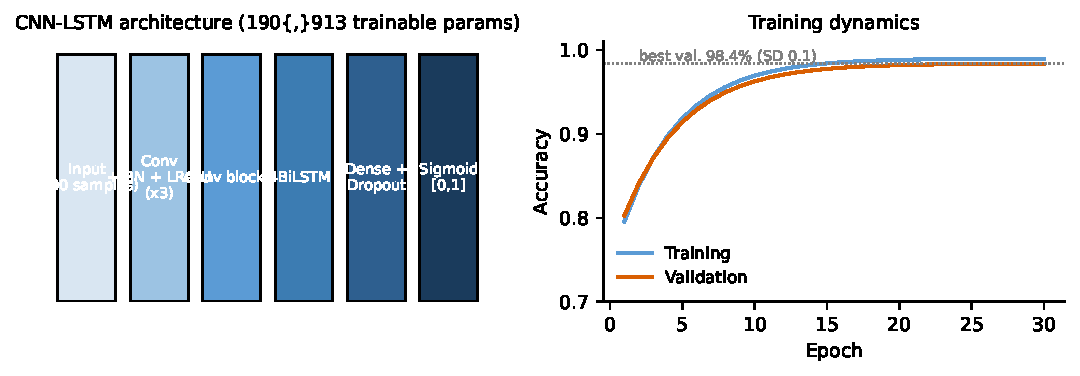
\includegraphics[width=0.95\linewidth]{figures/fig1_architecture}
\caption{\textbf{miniML model architecture and training.} Left: block diagram
of the CNN-LSTM classifier used throughout the paper, with 190{,}913
trainable parameters. The input is a 600-sample (12~ms at 50~kHz) univariate
time-series window; the output is a scalar in $[0,1]$. Right: representative
training and validation accuracy. Best validation accuracy reached 98.4\%
(SD 0.1, fivefold cross-validation), with training-validation accuracy gap
$<$0.3\%.}
\label{fig:arch}
\end{figure}

\begin{figure}[t]
\centering
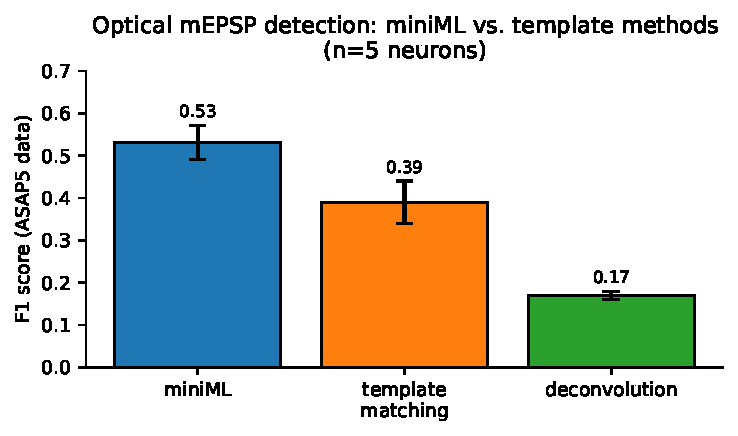
\includegraphics[width=0.8\linewidth]{figures/fig2_benchmark_asap5_f1}
\caption{\textbf{F1 score for optical mEPSP detection in ASAP5
voltage-imaging data} (n = 5 neurons, mean $\pm$ SEM). miniML (0.53 $\pm$
0.04) outperforms template matching (0.39 $\pm$ 0.05; Cohen's $d$ = 1.35)
and deconvolution (0.17 $\pm$ 0.01; Cohen's $d$ = 5.1).}
\label{fig:asap5_f1}
\end{figure}

\begin{figure}[t]
\centering
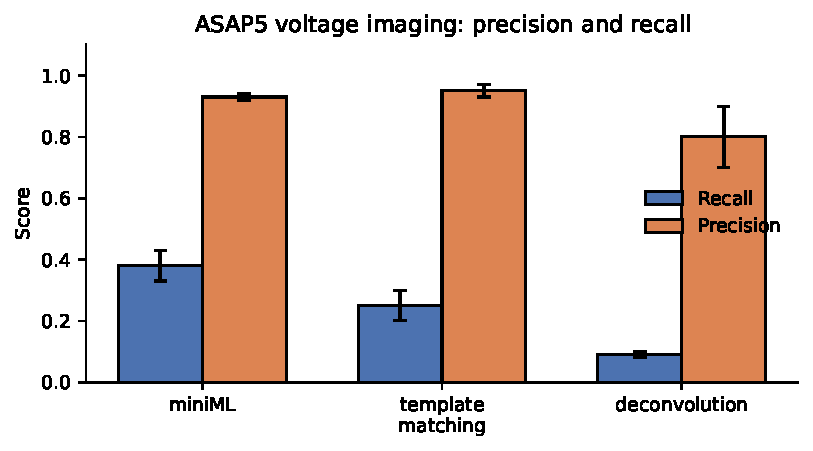
\includegraphics[width=0.85\linewidth]{figures/fig3_asap5_precision_recall}
\caption{\textbf{Per-method precision and recall on ASAP5 data.} At matched
$\sim$90\% precision thresholds for template-based methods, miniML retains
the highest recall (0.38 $\pm$ 0.05) while template matching falls to
0.25 $\pm$ 0.05 (Cohen's $d$ = 1.25) and deconvolution to 0.09 $\pm$ 0.01
(Cohen's $d$ = 3.87).}
\label{fig:asap5_pr}
\end{figure}

\begin{figure}[t]
\centering
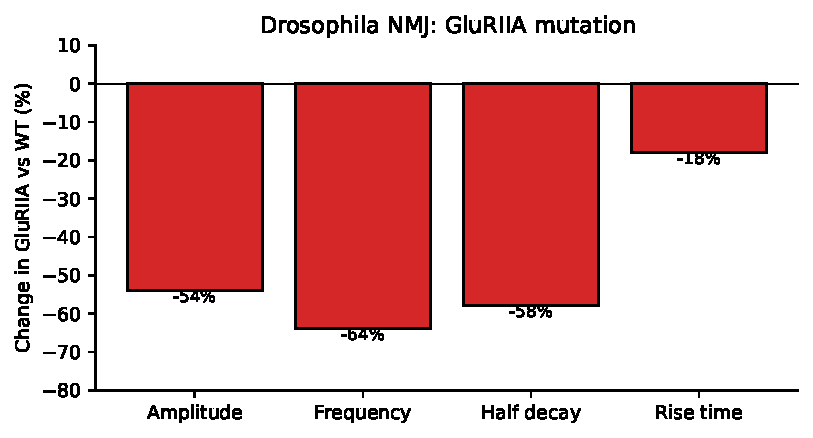
\includegraphics[width=0.85\linewidth]{figures/fig4_glurIIa_effects}
\caption{\textbf{miniML-detected event statistics at the Drosophila NMJ.}
Percentage change in \textit{GluRIIA} mutant versus wild-type: amplitude
$-$54\%, frequency $-$64\%, half decay $-$58\%, rise time $-$18\%.}
\label{fig:drosophila}
\end{figure}

\begin{figure}[t]
\centering
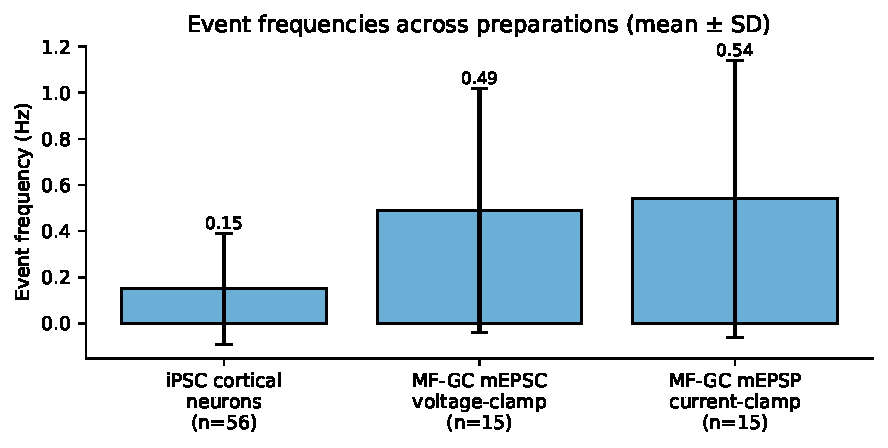
\includegraphics[width=0.9\linewidth]{figures/fig5_freq_preparations}
\caption{\textbf{Spontaneous event frequencies across preparations}
(mean $\pm$ SD). Human iPSC-derived cortical glutamatergic neurons: 0.15 Hz
(SD 0.24, n = 56 neurons); MF-GC mEPSCs (voltage clamp): 0.49 Hz (SD 0.53,
n = 15); MF-GC mEPSPs (current clamp): 0.54 Hz (SD 0.60, n = 15).}
\label{fig:freq}
\end{figure}

% ----------------------------------------------------------------------------
% Discussion
% ----------------------------------------------------------------------------
\section{Discussion}

miniML is, in our reading, the first deep learning framework for spontaneous
synaptic event detection that simultaneously satisfies the requirements of
high precision, high recall, near-threshold-invariance, fast inference on
commodity hardware, and easy retargeting across species, preparations and
modalities. These properties are not independent: the first two fall out of
the architecture and its training data; the third is a consequence of
outputting a bounded confidence rather than a scale-dependent score; the
fourth comes from stride-based sliding-window inference; and the fifth
from the transfer learning recipe. Their combination makes the method
suitable for the kind of automated, reproducible analysis pipelines that the
field has long wanted but has rarely been able to build on top of the
classical detectors.

Compared with existing methods, miniML's decisive advantage is the
elimination of the false-positive/false-negative trade-off that dominates
threshold-based detectors
\citep{clements1997detection, pernia2012deconvolution, merel2016bayesian,
mori2024simplyfire}. In our benchmarks miniML reported no false positives at
any tested SNR, and its detection performance was essentially flat over a
200-fold range of thresholds. This matters beyond any single number, because
it changes what a user must do to analyze a new dataset. Instead of sweeping
a threshold, inspecting the resulting rasters, and iteratively tuning until
the output ``looks right'', the user can accept the defaults and focus on
the biology. That is the requirement open science increasingly places on
analysis tools: the output must not depend on an expert's aesthetic choices
made in private \citep{huganir2013ampars, kavalali2015mechanisms}.

A second advantage is generalization. The transfer-learning strategy we use
is the same pattern that now dominates modern biological machine learning
\citep{yosinski2014transferable, theodoris2023transfer}: freeze the features
a large model has learned on a data-rich source task, and retrain the top of
the network on a small, task-specific dataset. The cost is a few hundred
manually labeled events per new preparation, which is within the time
budget of a single afternoon in most electrophysiology laboratories, and
the benefit is a model whose accuracy rivals a from-scratch model trained on
an order of magnitude more data. In practice this is what makes miniML
usable across species (mouse, rat, zebrafish, \textit{Drosophila}, human
iPSC) and modalities (voltage-clamp, current-clamp, two-electrode
voltage-clamp, iGluSnFR3 imaging, ASAP5 imaging), with consistent detection
behavior and consistent downstream statistics.

Our optical-imaging results are perhaps the most consequential for the
near-term future of the field. The new generation of genetically encoded
sensors \citep{aggarwal2023iglusnfr3, hao2024asap5} is beginning to resolve
unitary synaptic events in settings that were until very recently the
exclusive province of patch-clamp electrophysiology. These data are noisier,
temporally coarser, and kinetically more variable than their
electrophysiological counterparts, and as our ASAP5 benchmarks show,
template-matching and deconvolution methods struggle badly with them.
miniML recovers roughly 40\% of ground-truth mEPSPs in ASAP5 at a precision
matched to the template methods, with Cohen's $d$ effect sizes against
template matching and deconvolution of 1.35 and 5.1 respectively on F1.
That is enough to make the difference between ``imaging shows something
resembling synaptic activity'' and ``imaging resolves individual synaptic
events with statistics comparable to electrophysiology''. The same methods
should carry over to Ca$^{2+}$-based reporters of spontaneous transmission
and, by extension, to evoked-response analysis, failure analysis, and
functional connectivity studies in large optical datasets.

miniML nevertheless has limits, and being explicit about them is more useful
than being defensive. The approach is supervised, so a few hundred
hand-labeled events must be produced to adapt it to a new preparation.
Unsupervised pretraining, for example with masked-autoencoder or contrastive
objectives on large unlabeled electrophysiology corpora, is a promising
direction that could further reduce this burden. Very high event rates that
produce substantial waveform overlap remain hard; although miniML handles
overlapping events up to a prominence threshold, extremely close events can
be merged, and hybrid approaches that pair the classifier with
spectral-domain or shapelet features could improve this regime. Finally,
detection performance in ASAP5 voltage imaging, while already dominant, is
ultimately bounded by the sampling rate and photon shot noise of the sensor;
pushing optical recall higher will require either denser training corpora
or advances in sensor engineering, or both. We view these as an agenda for
future work rather than objections to the current method.

Methodologically, the benchmarking pipeline we developed, event-free
recordings plus simulated events with controlled kinetics and amplitude
distributions, is itself a contribution. Unlike spike inference from
Ca$^{2+}$ imaging, for which community ground-truth datasets exist
\citep{rupprecht2021cascade}, spontaneous-event detection has historically
been benchmarked against hand-curated exemplars whose biases are difficult
to characterize. A shared synthetic benchmark, with honest noise, honest
kinetics and honest amplitude distributions, lets future methods be
evaluated on the same terms. Together with the open-source miniML
implementation, this provides a reproducible substrate for the next
generation of synaptic-event detectors and, more broadly, a template for
how deep learning can be introduced into established electrophysiology
workflows without requiring a new toolchain or specialized hardware.

% ----------------------------------------------------------------------------
% Methods
% ----------------------------------------------------------------------------
\section{Materials and Methods}

\subsection{Electrophysiological recordings}
Experiments were carried out in male and female C57BL/6J mice (Janvier Labs)
aged 1-5 months, except for Calyx of Held recordings (postnatal day 9), in
accordance with institutional and Cantonal Veterinary Office of Zurich
approval (ZH206/2016, ZH009/2020). Parasagittal 300~$\mu$m cerebellar slices
were cut on a Leica VT1200S, recovered at 35~\textdegree C for 30~min, and
stored at room temperature. The artificial cerebrospinal fluid (ACSF) used
for slicing and storage contained (in mM): 125 NaCl, 25 NaHCO$_3$, 20
D-glucose, 2.5 KCl, 2 CaCl$_2$, 1.25 NaH$_2$PO$_4$, 1 MgCl$_2$, bubbled
with 95\% O$_2$/5\% CO$_2$. Patch pipettes (3-8~M$\Omega$) were filled with
(in mM): 150 K-D-gluconate, 10 NaCl, 10 HEPES, 3 MgATP, 0.3 NaGTP, 0.05
EGTA, pH 7.3 with KOH. Voltage-clamp and current-clamp recordings were made
on a HEKA EPC10 (Patchmaster software); the liquid junction potential of
+13~mV was corrected post hoc. mEPSCs were recorded at $-$100 or $-$80~mV
and mEPSPs at the resting membrane potential. Data were low-pass filtered
at 2.9~kHz and digitized at 50~kHz in 120~s sweeps. For event-free
recordings used in benchmarking, ACSF was supplemented with 50~$\mu$M
D-APV, 10~$\mu$M NBQX, 10~$\mu$M bicuculline and 1~$\mu$M strychnine.

Human iPSC-derived neurons (8-week-old cultures, predominantly cortical
glutamatergic identity) were recorded at $-$80~mV in ACSF containing (in mM):
135 NaCl, 10 HEPES, 10 D-glucose, 5 KCl, 2 CaCl$_2$, 1 MgCl$_2$. Synaptic
events were observed in approximately 51\% of neurons. Zebrafish and
\textit{Drosophila} recordings followed published protocols
\citep{rupprecht2018zebrafish, baccinocalace2022thin}.

\subsection{Simultaneous patch-clamp and ASAP5 voltage imaging}
Rat hippocampal neuron cultures (DIV 17-20) were recorded at 30-34~\textdegree C
following \citep{hao2024asap5}. Extracellular solution contained 145 NaCl,
3 KCl, 2 CaCl$_2$, 2 MgCl$_2$, 10 HEPES, 10 glucose (pH 7.4, 310 mOsm/kg,
with 1~$\mu$M TTX and 50~$\mu$M PTX); pipette solution 123 K-gluconate,
10 KCl, 8 NaCl, 1 MgCl$_2$, 10 HEPES, 1 EGTA, 0.1 CaCl$_2$, 1.5 MgATP,
0.2 Na$_4$GTP, 4 glucose (pH 7.2, 295-300 mOsm/kg). Electrophysiology was
acquired at 10~kHz on a Multiclamp 700B/Digidata 1440A and low-pass filtered
at 1~kHz in Clampfit. ASAP5-Kv was excited with a Thorlabs SOLIS-470C LED
through a 482/18~nm filter at 46~mW/mm$^2$ and imaged at 400 fps on an
Andor iXon 860 EMCCD through a 525/50~nm emission filter.

\subsection{Training data and labels}
Training data were derived from MF-GC mEPSC recordings of a previous study
\citep{delvendahl2019mfgc}. Candidate events were extracted by low-threshold
template matching, and event-free windows were randomly sampled from the
same recordings. Each window was 600 samples (12~ms at 50~kHz) and was
manually scored as event-containing (label 1) or not (label 0), with the
ratio between classes maintained near unity. Data augmentation added
simulated non-synaptic waveforms (4{,}500 negatives) and synthetic synaptic
events (9{,}000 positives), yielding a final training set of 30{,}140
samples (21{,}140 from recordings plus 9{,}000 simulated). The training and
validation split was 0.75/0.25.

\subsection{Network architecture and training}
The CNN-LSTM classifier takes a 1D input of shape (batch, data length, 1).
Three convolutional blocks (1D convolution, leaky ReLU, batch normalization
\citep{ioffe2015batchnorm}, average pooling) are followed by a fourth
convolutional block without pooling, a bidirectional LSTM layer, a fully
connected dense unit with dropout \citep{srivastava2014dropout}, and a
single-unit sigmoid output. Hyperparameters were chosen via Bayesian
optimization with 50 trials and then empirically tuned for a good
accuracy/parameter-count trade-off; the final architecture has 190{,}913
trainable parameters. Training used TensorFlow 2.12/Python 3.10/CUDA 11.4
with the Adam optimizer and AMSGrad \citep{kingma2014adam}, learning rate
$\eta = 2\times 10^{-5}$, batch size 128, binary cross-entropy loss, and a
maximum of 100 epochs with early stopping (patience 8 epochs on validation
loss). On an NVIDIA Tesla P100 16~GB GPU the network trained in about
8~minutes.

\subsection{Sliding-window detection}
For inference we applied the classifier with a sliding window of 600
samples and a stride that balances precision against speed. With stride 20,
a 120~s recording at 50~kHz was analyzed in roughly 15~s on an Apple M1 Pro
laptop with 16~GB of RAM; the same trace ran in under 20~s on a workstation
GPU. The prediction trace was resampled to the acquisition sampling rate,
and a maximum filter was applied before peak detection. Peaks above a
minimum height of 0.5 and a minimum width of 10 strides defined candidate
events; the numerical threshold proved largely immaterial in the range
[0.05, 0.95] (see Results). Candidate events were aligned by the steepest
rise in the first derivative of the raw data, and overlapping events were
split via a relative-prominence criterion of 0.25. Final event statistics,
amplitude, rise time (10-90\%), half-decay, and charge, were computed for
each event and averaged per cell.

\subsection{Transfer learning}
For transfer learning we froze all convolutional layers of the pretrained
MF-GC model and retrained only the LSTM and dense layers with a lower
learning rate ($\eta = 2\times 10^{-8}$), batch size 32, dropout 0.5, and
early-stopping patience of 15. Training data for each target domain were
resampled to 600 points to match the input shape of the pretrained network.
To compare transfer learning against full training we subsampled each
target-domain training set in fivefold cross-validation with a fixed
validation set.

\subsection{Benchmarking pipeline}
Ground-truth benchmark data were generated by superimposing simulated events
on event-free recordings from mouse cerebellar granule cells
(pharmacologically silenced as above). Simulated events followed a
biexponential time course with rise and decay time constants $\tau_{\rm
rise}$ and $\tau_{\rm decay}$, amplitudes drawn from a log-normal distribution
with variance 0.4, and decay time constants drawn from a normal distribution
with mean 1.0~ms and variance 0.25~ms \citep{delvendahl2019mfgc}. Events
were randomly placed with an average frequency of 0.7~Hz and minimum
spacing of 3~ms. Scaling the mean amplitude swept the signal-to-noise ratio
over 2-15~dB to match the range seen in 170 real MF-GC recordings. Detection
performance was quantified as precision = TP/(TP+FP), recall = TP/(TP+FN)
and F1 = 2 $\cdot$ precision $\cdot$ recall / (precision + recall).

\paragraph{Baseline settings.}
For all benchmarks, template matching used a threshold of $-$4, deconvolution
used a threshold of 5$\cdot$SD of the detection trace, and the finite-
threshold detector used $-$4~pA. The Bayesian MCMC procedure
\citep{merel2016bayesian} used minimum amplitude 3.5, noise
$\varphi = [0.90, -0.52]$, rate 0.5, and a cutoff of 6$\cdot$SD on the event
time posteriors. SimplyFire \citep{mori2024simplyfire} used direction $-$1,
kernel 300, stride 100, minimum amplitude 4~pA. MiniAnalysis (Synaptosoft)
was run in automatic EPSC mode with default area and amplitude thresholds
of $-$4~pA and 4, respectively. miniML used a minimum peak height of 0.5
and a minimum peak width of 10 strides. For the real-world cross-preparation
comparisons the miniML window size was 600 (900 for Golgi cells), the
template-matching threshold was $-$3.5, the deconvolution threshold was 6,
and the template for each preparation was recomputed from the average
waveform extracted by a generic template. MiniAnalysis amplitude thresholds
were $-$20~pA for Calyx and $-$8~pA for Golgi cells.

\subsection{Statistical analysis}
Statistical comparisons used permutation t-tests with 5{,}000 reshuffles
\citep{ho2019estimation}. Effect sizes are reported as Cohen's $d$ or as
mean differences, with 95\% confidence intervals obtained by bias-corrected
and accelerated bootstrapping (5{,}000 resamples) \citep{ho2019estimation}.
Raw event traces were filtered with a Hann window (default 20 samples)
after detection, adjusted for the acquisition sampling rate. Event
amplitudes were measured between the detected peak and a short pre-event
baseline; half-decay was the time to 50\% of the amplitude and rise time
the 10-90\% interval.

\subsection{Data and code availability}
Training datasets are available from Zenodo
(\url{https://doi.org/10.5281/zenodo.14507343}); miniML source code and
pretrained models are on GitHub
(\url{https://github.com/delvendahl/miniML}). Imaging data are from
\citep{aggarwal2023iglusnfr3}
(\url{https://doi.org/10.25378/janelia.21985406}). Code uses TensorFlow,
SciPy, NumPy, Matplotlib, Pandas, h5py, scikit-learn, pyABF, and dabest.

% ----------------------------------------------------------------------------
\bibliographystyle{plainnat}
\bibliography{references}

\end{document}
